\documentclass{article}
\usepackage{graphicx}
\usepackage[a4paper, total={16cm, 24cm}]{geometry}
\usepackage{xspace}
\usepackage[hidelinks]{hyperref}
\usepackage{color}
\newcommand{\p}{\texttt{phyloscanner}\xspace}
\newcommand{\pmt}{\texttt{phyloscanner\_make\_trees.py}\xspace}
\newcommand{\pat}{\texttt{phyloscanner\_analyse\_trees.R}\xspace}
\newcommand{\pcl}{\texttt{phyloscanner\_clean\_alignment.R}\xspace}
\let\c\texttt
\newcommand{\www}{\color{blue} \underline}
\newcommand{\R}{\c{RAxML}\xspace}

\title{\p\\available from \href{https://github.com/BDI-pathogens/phyloscanner}{\www{github.com/BDI-pathogens/phyloscanner}}}
\date{This manual last updated \today}
\author{Coding lead by Chris Wymant and Matthew Hall,\\with contributions from Oliver Ratmann and Christophe Fraser}

\begin{document}
\maketitle


\begin{figure}[!h]
\centering
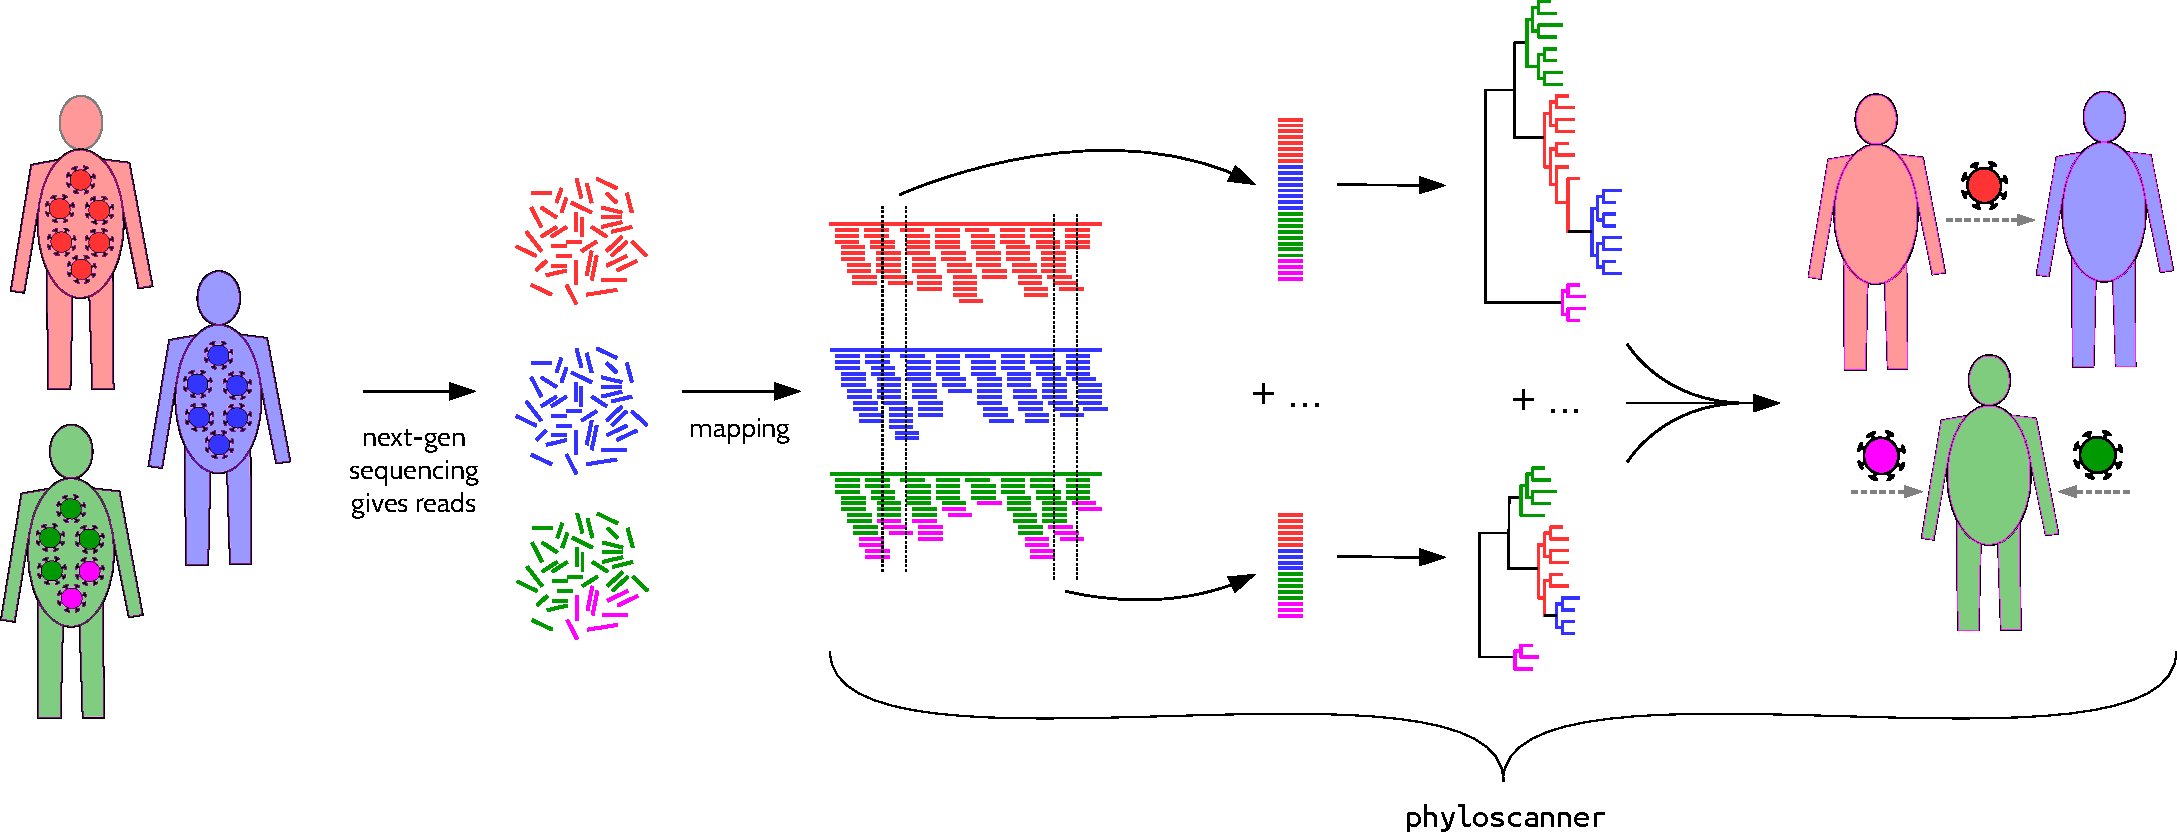
\includegraphics[width=0.95\textwidth]{PhyloscannerDiagram_big4.pdf}
\end{figure}

\vspace*{5mm}

\p analyses pathogen genetic diversity and relationships between and within hosts at once, in windows along the genome using mapped {\it reads} (fragments of DNA produced by next-generation sequencing), or using phylogenies with multiple sequences per host previously generated by the user via any method.
An example showing its action on simulated data (which is included with the code) can be seen at the GitHub repository linked to above.

\vspace*{5mm}

If you have a query about \p, ask it publicly at the \href{https://groups.google.com/forum/\#!forum/phyloscanner-users}{\www{google group}}.  
If you have a problem getting the code to run or think you've found a bug, please create a \href{https://github.com/BDI-pathogens/phyloscanner/issues}{\www{\it New issue}} on the GitHub repository.
The usual bug-reporting etiquette applies.
For non-trivial bugs, to allow us to reproduce the problem it's helpful to have input that causes the problem.
This needn't be all your data.
For example if one read in a bam file is causing a problem, you could make a new bam file containing only that read, allowing us to see the problem very quickly.
Isolate the problem as much as you can first -- help us to help you!
If you get an error when you run \p as part of a larger piece of code you've written yourself (e.g. a job submission script to a cluster), please don't make us debug that -- the error might be in your code rather than ours.
Isolate the problem to the relevant \p command.

\vspace*{5mm}

If you use \p, please cite it~\cite{Wymant157768} and its dependencies: \c{SAMtools}~\cite{Li08062009}, \c{MAFFT}~\cite{Katoh15072002}, \c{RAxML}~\cite{doi:10.1093/bioinformatics/btu033} and \c{ggtree}~\cite{MEE3:MEE312628}.
Details of these are found in the file \c{CitationDetails.bib} in \p's \c{InfoAndInputs} subdirectory.

\vspace*{5mm}

Throughout the manual we'll use {\it phylogeny} and {\it tree} interchangeably.
Forgive us.

\newpage
\tableofcontents
\newpage

\section*{A tool in two parts}
Conceptually, \p can be neatly split into two steps.
Firstly, inferring phylogenies that contain both within- and between-host diversity, in windows along the genome, using mapped reads as input.
Secondly, analysing those phylogenies or other similar ones (i.e. containing within- and between-host diversity, but created however the user likes) in order to infer interesting things like transmission and multiply infected individuals, and give summaries of diversity.

This conceptual split is reflected in the code: \pmt runs the first step and \pat runs the second step.
Why didn't we merge the two steps into one?
\begin{itemize}
\item For some uses, step one may not be needed.
For example if you don't have mapped reads, but have sequence data in another format.
We presented an example of this in the \p paper: a dataset consisting of multiple whole genomes of {\it Streptococcus pneumoniae} for each person carrying the bacterium, obtained by separately sequencing multiple colonies.
\item For some uses, step two may not be needed.
Having extracted the within- and between-host diversity information in each window (first as a multiple sequence alignment and then as a phylogeny), you might want to do your own totally different analysis of it.
%Step one consists of extracting the right reads from all samples for each window, processing them, aligning them, then running \c{RAxML} on the aligned reads.
\item Each step is controlled by parameters and options to tailor its usage to different kinds of data, and we don't (yet) have a way to automatically optimise these for each data set, so you will need to have a little play to explore what's appropriate in your case.
If you are running both steps, it's best to think first about getting step one right first, and then getting step two right.
Step one is primarily about bioinformatics, step two about phylogenetic analysis.
\end{itemize}

Note that to run either \pmt or \pat, like running any executable file, you must either specify the full path to the executable (e.g.\\\c{/path/to/my/phyloscanner/code/}\pmt) or add the directory that contains the executable to the \c{\$PATH} environment variable in your terminal (google this if needed).
In the manual we'll refer to scripts named like \c{tools/SomeCode}; such scripts live in the \c{tools} subdirectory inside the main \p code directory.


Fun fact: step one was written by Chris, step two mostly by Matthew.
We sat next to each other while coding, and we hope that's reflected in how easy it is to make the two steps work together.
If it isn't, let us know.
%While the two steps can be run separately, we had their combined use  


\part{Inferring within- and between-host phylogenies in windows along the genome, using mapped reads}

\section{The basic command} \label{sec:The basic command}

As input to \pmt, you need to have generated files of mapped reads in bam format -- bam files henceforth.
The bam format does not include the sequence to which the reads were mapped -- the {\it reference} -- which we also need.
With the initial \c{\$} traditionally indicating that what follows is a command to be run on the command line / in a terminal (i.e. don't type that initial \c{\$}), the basic \pmt command looks like

\begin{verbatim}
$ phyloscanner_make_trees.py ListOfMyInputFiles.csv --windows 1,300,301,600,...
\end{verbatim}
where
\begin{itemize}
\item \c{ListOfMyInputFiles.csv} is a plain-text, comma-separated-variable (csv) format file in which the first column contains the bam files, the second column contains the corresponding reference files.
An optional third column, if present, contains {\it aliases} -- things to rename each bam file to in \pmt output; if not present the base name of the bam, i.e. the file name not including the directory path, will be used.
e.g. This input file list might look like\\
\c{PatientA.bam,PatientA\_ref.fasta,A\\
PatientB.bam,PatientB\_ref.fasta,B}\\
Bam file base names, and aliases if present, must be unique and free of whitespace.
Quotation marks are interpreted as wrapping/protecting fields, allowing them to contain commas that are not field separators.
You can generate this input file list however you like, including manually.
The following block of code illustrates how you might generate it automatically from the command line.
It also checks that your files exist, which \pmt does anyway, but it's always best to catch your errors soonest.
\begin{verbatim}
$ for ID in PatientA PatientB PatientC; do
$   bam=MyBamsDir/"$ID".bam
$   ref=MyRefsDir/"$ID".fasta
$   if [[ ! -f "$bam" ]]; then
$     echo "$bam does not exist" >&2
$     break
$   elif [[ ! -f "$ref" ]]; then
$     echo "$ref does not exist" >&2
$     break
$   fi
$   echo "$bam","$ref","$ID"
$ done > MyPhyloscannerInputFile.csv
\end{verbatim}
If those IDs were stored in a plain-text file \c{MyIDs.txt} separated by whitespace, you could replace the first line of that loop with\\
\c{for ID in \$(cat MyIDs.txt); do}
\item The \c{--windows} (or \c{-W}) option is used to specify an even number of comma-separated positive integers: these are the coordinates of the windows to analyse, interpreted pairwise, i.e. the first two are the left and right edges of the first window, the third and fourth are the left and right edges of the second window, $\ldots$ i.e. in the above example we have windows 1-300, 301-600, $\ldots$
\end{itemize}
You shouldn't run multiple \pmt commands simultaneously in the same directory, as it writes to and reads from files with fixed names, so the commands could clash.
If you're running multiple jobs in parallel on a computing cluster that starts jobs in the same place, ensure that each job runs in a different directory (e.g. using the \c{mkdir} and \c{cd} commands to make and change into a directory specific to that job).

\subsection{The Python version you use}
Note that \pmt can either be run like this:\\
\pmt\c{ [input and options]}\\
or like this:\\
\c{python }\pmt\c{ [input and options]}\\
In the former case, the version of Python used to execute \pmt is whatever version gets called when you simply run the command \c{python} in the terminal.
In the latter case, you can explicitly replace \c{python} by a specific version of Python on your machine, for example \c{python2.7} or \c{/usr/bin/python}.
The version of Python that's used must (a) be Python 2, not Python 3, and (b) contain the Python dependencies described in \mbox{\c{phyloscanner/InfoAndInputs/InstallationNotesForMakingTrees.sh}}.

\section{What do the window coordinates mean exactly?} \label{sec:CoordMeaning}
By default the references used for mapping, together with any extra references if included using the \c{--alignment-of-other-refs} option, are all aligned together and window coordinates are interpreted with respect to the alignment (i.e. position $n$ refers to the $n$th column of that alignment, which could be a gap for some of the sequences).
This alignment can be found in the file \c{RefsAln.fasta} after running \pmt, should you want to inspect it and possibly run again.
You can manually specify window coordinates with respect to this alignment, using the \c{--windows} option, or have windows automatically chosen using \c{--auto-window-params}, which attempts to minimise the affect of insertions and deletions in the references on your window width and overlap preferences.
Alternatively, if you are using the \c{--alignment-of-other-refs} option to include extra references, you can use \c{--pairwise-align-to} to name one of these references to be a kind of {\it reference reference}: instead of aligning of all the bam file references to each other, they will be sequentially and separately pairwise-aligned to your named reference, and window coordinates are interpreted with respect to that named reference (i.e. position $n$ refers to the position of the $n$th base of the named reference, not counting any gaps inside the reference).
Using the \c{--pairwise-align-to} option is expected to more stable than \c{--windows} or \c{--auto-window-params} if your bam file references are many and diverse, since pairwise alignment is easier than multiple sequence alignment.
It also has the advantage that when running \pmt more than once with different bam files, the coordinates mean the same thing each time.

\section{What windows should I choose?}
I'm glad you asked.
It's important.

\subsection{Start \& end}

You might as well fully cover the genomic region you're interested in.
That requires choosing where to start and where to end.
If you're interested in the whole genome, the start is 1 and the end is the genome length, or more precisely the length of the alignment of all references together (or the length of your named reference if you used the \c{--pairwise-align-to} option).
You may know that your reads don't start right at the beginning of the genome.
If this is the case, a good place to start your first window would be the genome position at which you start having reads.

If your reads were generated by amplifying the sample using primers, the primers should ideally have been trimmed from the reads as part of whatever bioinformatic pipeline produced your input bam files.
(This can be done for example using \href{https://github.com/sanger-pathogens/Fastaq}{\color{blue} \underline{\c{fastaq}}}, which is called as part of the \href{https://github.com/ChrisHIV/shiver}{\c{\color{blue} \underline{shiver}}} pipeline.)
Then a sensible choice for the start of the first window would be the first position after the first primer, and a sensible choice for the end of the last window would be the last position before the last primer.

{\it You might as well fully cover the genomic region you're interested in.}
Let's revisit that.
In what part of the genome would you like to do phylogenetics?
Perhaps all of it.
Then again, remember that phylogenetics assumes neutral evolution at every included site.
Though \pmt allows individual specified sites to be excised after alignment of all the reads from all the bam files, there may be regions of the genome where selected sites are so dense that it's simpler to skip the region altogether.
There may also be regions of the genome where there are so many insertions and deletions (indels) that you're sceptical that the reads will align correctly in the first place.
You can choose to specify no windows covering such regions.

\subsection{Window width} \label{sec:WindowWidth}
As well as choosing where your first window should start and where your last one should end, you need to choose how wide each window is.
On the one hand, increasing the width of a window increases its phylogenetic resolution.
To see this effect using just some existing reference sequences (forgetting momentarily about any read data you have), the script \c{tools/CalculateTreeSizeInGenomeWindows.py} could be useful: it calculates trees from references in sliding windows along the genome.
(It then calculates patristic distances, for a purpose discussed later in section~\ref{sec:normalisation}.)
You may be able to see from visual inspection, or from some automated analysis of your own, that one's ability to construct well-resolved phylogenies increases with window width.
On the other hand, a read must fully span a window to be included in it, so the wider you make a window the fewer reads it will contain.
To quantify this effect, you can run
\begin{verbatim}
$ tools/EstimateReadCountPerWindow.py ListOfMyInputFiles.csv
\end{verbatim}
(where \c{ListOfMyInputFiles.csv} is the same file as we discussed at the top of section~\ref{sec:The basic command}).
This command uses the information in each bam about the number of reads and how long\footnote{
In this particular instance we define read length as the length of the mapping reference covered by the read, from its start to its end.
This can differ from the actual read length due to insertions or deletions in the read relative to the reference.
Defining the read length this way is appropriate since we're interested in reads spanning windows, and windows get defined relative to the reference.
This length will also differ from the nominal read length of your sequencing run (which is typically one fixed value) if the reads have been trimmed as part of bioinformatic processing, e.g. removing primers, adapters, low-quality bases, or bits of the read that could not be mapped.
} they are; it then estimates the number of reads expected to span a window of width $W$ by assuming reads are distributed randomly over the whole genome (ignoring the actual read location information in the bam files).
If reads are found to be paired, the calculation is also done in the context of \pmt's \c{--merge-paired-reads} option, which merges each pair of reads into a single longer read if they overlap with each other (this will give exactly the same result as considering reads separately if reads in a pair never overlap).
The calculation is done as a function of $W$, showing how the number of reads decreases monotonically\footnote{
The number of positions at which we could place a window of width $W$ equals the length of the reference $- W + 1$.
The number of positions at which we could place a window of width $W$ such that it is wholly inside a read is the length of the read $- W + 1$.
The probability of a randomly placed read overlapping a window of width $W$ is therefore (read length $- W + 1$) / (reference length $- W + 1$).
The number of reads and their different lengths are fixed in the data; increasing $W$ will decrease this probability (except for reads that span the entire reference).}.
A good choice of window width, roughly, would be as large as you can get before the number of reads per window gets too low to make useful within-host phylogenies.
Skip ahead to section~\ref{sec:overlap} if that's good enough for you and you don't want to think about it any more.

The \c{--explore-window-widths} option of \pmt was written with the following balancing act in mind.
If a window is too wide, too few reads overlap it, as discussed.
However if it is too small, there aren't enough positions at which a variant can be observed and so few {\it unique} reads will be observed in the window.
Somewhere between these two extremes therefore maximises the number of unique reads.
The \c{--explore-window-widths} option reports, for each in a list of window widths to try, how many unique reads are found in each bam and in each successive along the genome.
To summarise these read counts into a single value that varies with window width, you could use the mean or the median, or you might be interested in a percentile lower than the 50th, if your concern is ensuring some minimal amount of diversity across all bams and all genomic positions.
Up to you.
Anecdotally, I did not find this option useful for our HIV data: manually examining phylogenies revealed that they were more interesting when a larger window width was used than the one that maximised the number of unique reads.

(Note that some of the other options can affect how many reads you get in a window and so can affect what \c{--explore-window-widths} will tell you, namely the \c{--excision-coords}, \c{--merging-threshold}, \c{--min-read-count}, \c{--quality-trim-ends}, \c{--min-internal-quality}, and \c{--discard-improper-pairs} options.
The first two can result in two or more unique reads being merged into one; the rest can simply discard some reads.
You could choose values for the associated parameters immediately and then use \c{--explore-window-widths}, or else come back to \c{--explore-window-widths} later on once you've got the hang of \pmt and investigated the effect of those other options in your data.)  

Power users might want to optimise their own measure of phylogenetic information as a function of window width; one of the first metrics to pop into your head might be the mean bootstrap of all nodes in the tree.
That's not advised because within a sample there may be many very similar sequences, and the set of nodes connecting these may have poor bootstrap support, but this is not something that ought to be penalised.
Also in theory you might be able to increase the window width until only a single read is found spanning the window in each patient; your bootstraps might then be great, because between-host diversity is greater than that within-host, but you've thrown out all the within-host information.


\subsection{Window overlap} \label{sec:overlap}
How much should neighbouring windows overlap?
\begin{itemize}
\item A good, simple answer to this is zero, i.e. each window starts right after the previous one ends.
e.g. 1-99, 100-199, 200-299, $\ldots$
\item Negative overlap means unused space in between windows, e.g. 1-99, 200-299, 400-499, $\ldots$
The only reason for this is if you want to exclude certain parts of the genome.
(Though it's hard to imagine that the regions you want to exclude are perfectly regularly spaced.)
\item Positive overlap means the next window begins before the current one ends, e.g. 1-99, 50-149, 100-199, $\ldots$
There's a redundancy in doing this, because you're analysing the same information multiple times.
However there's a little bit of stochasticity involved when performing algorithmic multiple sequence alignment then phylogenetic inference, so even if two windows overlap heavily some minor differences in the results could arise by chance.
Positive overlap may therefore smooth out some of this stochasticity, at the expense of additional compute time.
(You'll also need to take into account the non-independency of overlapping windows if you interpret results from multiple windows in a probabilistic framework.)
 
 \end{itemize}

\section{What output files are produced?}

By default, those files that are produced for each window are grouped into subdirectories by file type.
\begin{itemize}
\item \c{RefsAln.fasta}.
This contains the mapping reference from each bam file, together with any extra references included with \c{--alignment-of-other-refs}.
This alignment is not created if \c{--pairwise-align-to} is used.
\item \c{AlignedReads/AlignedReadsInWindow\_X\_to\_Y.fasta} (where $X$ and $Y$ are window coordinates).
Contains the reads from all bam files in the window $X$-$Y$, after processing and alignment, but before excision of any positions specified with \c{--excision-coords}.
Reads are automatically assigned a name of the form {\it A\_read\_M\_count\_N}, where {\it A} identifies the bam from which the read came, $N$ is the number of times that read was found (either identical copies of the same sequence, or merged similar sequences if \c{--merging-threshold} is used), and $M$ is the rank of the read when they are ordered by count (i.e. $M=1$ is the most common read, $M=2$ the second most common etc.)
\item \c{AlignedReads/AlignedReads\_PositionsExcised\_InWindow\_X\_to\_Y.fasta}.
Only produced if you specified some positions to excise with \c{--excision-coords}, and at least one of those positions was inside\footnote{
Note that if \c{--pairwise-align-to} is used, the window coordinates $X$ and $Y$ mean the same thing as the excision coordinates.
If \c{--pairwise-align-to} is {\it not} used, the window coordinates $X$ and $Y$ mean positions $X$ and $Y$ in \c{RefsAln.fasta} as discussed in section~\ref{sec:CoordMeaning}; therefore a position to excise, $Z$, being inside the window $X$-$Y$ is not the same as $X\leq Z \leq Y$.
} the window $X$-$Y$.
If this file exists, the tree in window $X$-$Y$ is based on this alignment (not \c{AlignedReadsInWindow\_X\_to\_Y.fasta}).
Note that excising positions may result in reads that were previously distinct becoming identical -- if they differed only at the excised positions.
This is checked after positions are excised, and reads from the same bam that have become identical are merged with an updated count.
Similarly, if the merging of similar reads (in addition to identical reads) has been specified, the merging is rerun after excision of positions.
If the excision of positions results in reads becoming merged, clearly there will not be a one-to-one correspondence between reads before and after excision: after merging there may be fewer unique reads, though with the same total count.
\item \c{Consensuses/Consensuses\_InWindow\_X\_to\_Y.fasta}.
In this alignment, the set of unique reads retained from each bam file is collapsed into a single sequence: their consensus (taking the most common base/gap at each position, weighting each unique read by its count).
Note that in general this consensus could differ from the corresponding part of a consensus called using all reads mapped along the full length of the reference, because the only reads retained by \pmt in a window are those fully spanning it.
This process can result in some columns containing only gaps; these columns are kept, so that the coordinates of this file match those of \\\c{AlignedReadsInWindow\_X\_to\_Y.fasta}.
\item \c{Consensuses/Consensuses\_PositionsExcised\_InWindow\_X\_to\_Y.fasta}.
The consensus as previously, but with any specified positions to excise excised.
Only produced if there are such positions.
\item \c{DiscardedReads/DiscardedReads\_A.bam}, where A identifies one of the input bams.
Only produced if \c{--inspect-disagreeing-overlaps} is used; see that option's description in ~\ref{sec:BioinfArgs}.
These files will be accompanied by \c{DiscardedReads\_A\_ref.fasta} (the reference for the bam file).
\item \c{DuplicationData/DuplicateReadCountsRaw\_InWindow\_X\_to\_Y.csv}.
Each row in this csv-format file corresponds to one instance of exactly the same unique read being found in two different bams, {\it before} any processing of the reads (merging, excising positions etc.).
The first two columns show the two bams involved, and the third and fourth columns show the count of the read in the two bams.
If a read is exactly duplicated in $N$ different bams, then there will be $N(N-1)/2$ associated lines in this file -- one for each different pair of bams.
See also the information in the next point.
These files will not be produced if \c{--dont-check-duplicates} is specified.
\item \c{DuplicationData/DuplicateReadCountsProcessed\_InWindow\_X\_to\_Y.csv}.
Each row in this csv-format file corresponds to one instance of exactly the same unique read being found in at least two different bams, {\it after} all processing of the reads (merging, excising positions etc.).
If the same read is found in $N$ different bams, there will be one row for this, containing $N$ fields separated by commas (each row in general therefore has a different number of columns, though 2 is the most common).
Each field is the name of the read, assigned based on the bam in which it was found.
These files will not be produced if \c{--dont-check-duplicates} is specified.\\
Why is information about the duplication of reads checked and recorded twice, in these two different files?
Duplication information {\it after} processing is easiest to work with, because it is the processed reads that are used to infer phylogenies.
However instances of exact duplication {\it before} any processing of the reads is a better indicator of cross-sample contamination.
Firstly because the options for similarity-based merging of reads within each bam, and for a minimum read count for inclusion, result in fewer unique reads to compare between bams.
Secondly because excising positions makes reads shorter and increases the possibility for genuine cross-sample duplication (i.e. not contamination).
Anecdotally, we found that being trigger-happy with deleting all codons associated with HLA escape in a conserved part of the HIV genome resulted in considerable duplication in the reads after processing that was not present before.
Note that during both similarity-based merging of reads and excision of positions (which is followed by merging newly identical reads), we lose track of the original identity of reads, i.e. we don't know what the correspondence is between reads before processing and after processing.
\item \c{DuplicationData/DuplicateReads\_contaminants\_InWindow\_X\_to\_Y.fasta}.
Only produced if \\\c{--contaminant-count-ratio} is used; see that option's description in section~\ref {sec:DeprecatedArgs}.
\item \c{ReadNames/ReadNames1\_InWindow\_X\_to\_Y\_InBam\_A.txt}.
Only produced if \c{--read-names-1} is used; see that option's description in section~\ref{sec:BioinfArgs}.
\item \c{ReadNames/ReadNames2\_InWindow\_X\_to\_Y\_InBam\_A.csv}.
Only produced if \c{--read-names-2} is used; see that option's description in section~\ref{sec:BioinfArgs}.
\item \c{RecombinationData/RecombinantReads\_InWindow\_X\_to\_Y.fasta}.
Only produced if \\\c{--check-recombination} is used; see that option's description in section~\ref{sec:RecArgs}.
\end{itemize}
Some temporary files are also written to the working directory; by default these are deleted.
(They are kept with \c{--keep-temp-files}.)

\section{Optional arguments}

Information about all optional arguments and what they do can also be seen by running \\\pmt with the \c{--help} option.
That will give information guaranteed to be synchronised to your current version of the code, as well as showing all option shorthands (e.g. \c{--help} = \c{-h}); however we go into slightly more detail here.
We particularly encourage you to familiarise yourself with the {\it Window options} and {\it Recommended options} below, which are particularly important for running \pmt well.

\subsection{Window options}
You must choose exactly one of these: \c{--windows}, \c{--auto-window-params}, \c{--explore-window-widths}.
\begin{itemize}
\item \c{--windows}: used to specify a comma-separated series of paired coordinates defining the boundaries of the windows.
e.g. specifying \c{1,300,301,600,601,900} would define windows 1-300, 301-600, 601-900.
\item \c{--auto-window-params}: used to specify 2, 3 or 4 comma-separated integers controlling the automatic creation of regular windows.
\begin{itemize}
\item The first integer is the width you want windows to be.
If the \c{--pairwise-align-to} option is {\it not} being used, we create an alignment containing all references, as mentioned already.
In this case, we weight each column in this alignment by its non-gap fraction, so that windows in which many references have gaps become correspondingly wider.
If the \c{--pairwise-align-to} option {\it is} being used, width is simply interpreted with respect to the named reference (i.e. a width of $W$ means each window contains $W$ bases from that reference).
\item The second is the overlap between the end of one window and the start of the next.
This can be negative, implying unused space in between windows; the recommended value of 0 means each window starts right after the previous one ends.
\item The third integer, if specified, is the start position for the first window.
If not specified, this is 1.
\item The fourth integer, if specified, is the end position for the last window.
If not specified, windows will continue up to the end of the reference or references.
\end{itemize}
\item \c{--explore-window-widths}: use this option to explore how the number of unique reads found in each bam file in each window, all along the genome, depends on the window width.
After this option specify a comma-separated list of integers.
The first integer is the starting position for stepping along the genome, in case you're not interested in the very beginning.
Subsequent integers are window widths to try.
For example, if you specified 1000,100,150,200 we would count the number of unique reads in windows 1000-1099, 1100-1199, 1200-1299, ... and in 1000-1149, 1150-1299, 1300-1449 ... and in 1000-1199, 1200-1399, 1400-1599, ... where the dots denote continuation to the end of the genome.
Output is written to the file specified with the \c{--explore-window-width-file} option.
\item \c{--explore-window-width-file}: used to specify an output file for window width data, when the \c{--explore-window-widths} option is used.
Output is in csv format.
\end{itemize}

\subsection{Recommended options} \label{sec:RecArgs}
%Options we think are particularly worth your while understanding and using.
\begin{itemize}
\item \c{--alignment-of-other-refs}: used to specify an alignment of reference sequences for inclusion with the reads, for comparison.
These references need not be those used to produce the bam files.
This option is required if \p is to analyse the trees it produces (i.e if you are going to run \pat after \pmt).
The full set of processed, unaligned reads extracted from each window are aligned to the corresponding section of the reference alignment using \c{mafft --add}.
\item \c{--pairwise-align-to}: by default, \pmt figures out where corresponding windows are in different bam files by creating a multiple sequence alignment containing all of the mapping references used to create the bam files (plus any extra references included with \c{--alignment-of-other-refs}), and window coordinates are interpreted with respect to this alignment.
However using this option, the mapping references used to create the bam files are each separately pairwise aligned to one of the extra references included with \c{--alignment-of-other-refs}, and window coordinates are interpreted with respect to this reference.
The reference to use should be specified after this option.
Using this option is necessary if you want to run the \c{tools/CalculateTreeSizeInGenomeWindows.py} script and feed its output into \pat via its \c{--normRefFileName} option (see )
\item \c{--x-raxml}: use this option to tell \pmt how to run \R, including both the executable (with the path to it if needed), and the options.
If you do not specify anything, we will try to find the fastest \R exectuable available (first \c{raxmlHPC-AVX}, then \c{raxmlHPC-SSE3}, then \c{raxmlHPC}) and use the options \c{-m GTRCAT -p 1 --no-seq-check}.
You will need to specify something if the path to your \R executable is not contained in your \c{PATH} environment variable (i.e. if you need to specify the path to the executable in order to run it), or if you want to use different \R options.
\c{-m} tells \R which evolutionary model to use, and \c{-p} specifies a random number seed for the parsimony inferences; both are compulsory.
You may include any other \R options in this command (including multi-threading, provided you use one of the multi-threaded executables).
The set of things you specify with \c{--x-raxml} need to be surrounded with one pair of quotation marks (so that they're kept together as one option for \pmt and only split up for \R).
If you include a path to your \R executable, it may not include whitespace, since whitespace is interpreted as separating \R options.
Do not include options relating to bootstraps: use \pmt's \c{--num-bootstraps} and \c{--bootstrap-seed} options instead.
Do not include options relating to the naming of files.
\item \c{--merge-paired-reads}: this is only relevant for paired-read data for which the mates in a pair
(sometimes) overlap with each other, but is very useful for such data.
With this option, overlapping mates in a pair are merged into a single (longer) read.
This allows wider windows to be used, enhancing the phylogenetic resolution in a single window.
Pairs will only be merged if they agree on the bases in the overlap and where they have been mapped to; if the reads disagree, that pair is discarded.
Discarded pairs can be inspected by using \c{--inspect-disagreeing-overlaps}.
If reads are paired but never overlap, trying to merge them will do nothing except increase \pmt's run time and memory usage; if you're not sure about read pair overlap (i.e. you don't know the {\it insert size distribution} for your data), run \\\c{tools/EstimateReadCountPerWindow.py} as discussed at the start of section~\ref{sec:WindowWidth}.
\item \c{--check-recombination}: calculate a metric of recombination for each sample's set of reads in each window.
(Recommended only if you're interested, of course.)
How the metric is calculated: for each possible set of three sequences, one is considered the putative recombinant and the other two the parents.
For each possible crossover point (the point at which recombination occurred), we calculate $d_L$ as the difference between the Hamming distance from the recombinant to one parent and the Hamming distance from the recombinant to the other parent, looking to the left of the crossover point only; similarly we calculate $d_R$ looking to the right of the crossover point only.
$d_L$ and $d_R$ are signed integers, such that their differing in sign indicates that the left and right sides of the recombinant look like different parents.
We maximise the difference between $d_L$ and $d_R$ (over all possible sets of three sequences and all possible crossover points), take the smaller of the two absolute values, and normalise it by half the length of the alignment of sequences.
The resulting metric is constrained to be between 0 and 1, inclusive.
The maximum possible score of 1 is obtained if and only if the two parents disagree at every site, the crossover point is exactly in the middle, and either side of the crossover point the recombinant agrees perfectly with one of the parents e.g.\\
AAAAAAA\\
AAAACCC\\
CCCCCCC\\
Calculation time scales cubically with the number of unique sequences each sample has per window, and so the option is turned off by default.
You can save time by only turning it on only after you've settled on the values of other parameters that affect the number of unique sequences per window (notably window width, a merging threshold and a minimum read count).
\end{itemize}

\subsection{Read quality options}
\begin{itemize}
\item \c{--discard-improper-pairs}: discard all reads that are were flagged, at the time of mapping, as improperly paired: in the wrong orientation, or one mate unmapped, or too far apart.
For paired-read data.
\item \c{--quality-trim-ends}: used to specify a quality threshold for trimming the ends of reads.
We trim each read inwards until a base of this quality is met.
\item \c{--min-internal-quality}: used to specify an internal quality threshold for reads.
Reads are allowed at most one base below this quality; any read with two or more bases below this quality are discarded.
(If used in conjunction with the \c{--quality-trim-ends option}, the trimming of the ends is done first.)
\item \c{--min-read-count}: used to specify a minimum count for each unique read.
Reads with a count (i.e. the number of times that sequence was observed, after merging if merging is being done) less than this value are discarded.
The default value of 1 means all reads are kept.
You might want to discard rare reads to protect against sequencing error.
Retaining fewer reads will also speed up all subsequent processing and analysis of the reads.
\end{itemize}

\subsection{Other assorted options}
\begin{itemize}
\item \c{--excision-coords}: used to specify a comma-separated set of integer coordinates that will be excised from the aligned reads before phylogenies are made.
Useful for sites of non-neutral evolution, which distort phylogenies.
Requires the \c{--excision-ref} flag.
\item \c{--excision-ref}: used to specify the name of a reference (which must be present in the file you specify with \c{--alignment-of-other-refs}) with respect to which the coordinates specified with \c{--excision-coords} are interpreted.
If you are also using the \c{--pairwise-align-to} option, you must specify the same reference there
and here.
\item \c{--merging-threshold-a}: when multiple reads in the same bam file have exactly the same sequence, \pmt always collapses these to a single read with an associated {\it count} (i.e. the number of times that exact sequence was found in distinct reads in the bam file).
With this option, similar reads are merged as well as identical reads.
Use this option to specify a positive integer as the threshold for merging.
If read X differs from read Y by this threshold or less, and X has the smaller count, we keep only read Y and update its count to be the sum of the two counts.
Note that with \c{--merging-threshold-a}, if X is similar enough to Y for merging, but Y has already been merged into Z, X will only be merged into Z too if X and Z are similar enough (contrast with \c{--merging-threshold-b} below).
What this algorithm does is to start with the most common read, see if any less common reads are similar enough to into it, and if so remove those reads and use their count to bolster the more common read.
The procedure is repeated starting with the second most common read, skipping any reads that have already been `used up'  in merging; then the third most common read and so on.
\item \c{--merging-threshold-b}: similar to \c{--merging-threshold-a} above, except that if X is similar enough to Y for merging, but Y has already been merged into Z, X will automatically be merged into Z.
This algorithm effectively partions the set of reads into groups such that each member of a group is similar enough to at least one other group member (and each group can be split no further, i.e. no read is similar enough to any read outside its own group), and uses only the read with the highest count to represent each group.
For the same value of the threshold, merging \c{b} will merge as much or more than merging \c{a} (i.e. \c{b} will tend to result in fewer unique reads).
\item \c{--num-bootstraps}: used to specify the number of bootstraps to be calculated for \c{RAxML} trees (by default, none, i.e. only the maximum-likelihood tree is calculated).
\item \c{--bootstrap-seed}: used to specify the random-number seed for running \c{RAxML} with bootstraps.
The default is 1.
\item \c{--output-dir}: used to specify the name of a directory into which output files will be moved.
If it does not exist, it will be created; however we cannot create a new directory inside a directory that does not yet exist.
Temporary and output files are always created in the working directory, i.e. the directory in which the \pmt command was run, but with this option the output files are copied to the specified directory at the end.
\item \c{--time}: print the times taken by different steps.
\item \c{--x-mafft}: used to specify the command you need in order to run \c{mafft}.
The default is simply \c{mafft}; if your \c{mafft} executable is not in the \c{\$PATH} environment variable for your terminal (google this if you don't know what it means) you will need to include the directory where this executable lives, e.g. \c{/path/to/where/I/installed/mafft/mafft}.
\item \c{--x-samtools}: used to specify the command you need in order to run \c{samtools}.
The default is simply \c{samtools}.
See the points raised for the \c{--x-mafft} option above.
\item \c{--keep-output-together}: by default, subdirectories are made for different kinds of output.
With this option, all output files will be in the same directory (either the working directory, or whatever you specify with \c{--output-dir}).
\item \c{--keep-temp-files}: keep temporary files we create on the way (these are deleted by default).
\end{itemize}

\subsection{Options for bioinformatic interrogation} \label{sec:BioinfArgs}
Options for detailed bioinformatic interrogation of the input bam files, not intended for normal usage.
\begin{itemize}
\item \c{--inspect-disagreeing-overlaps}: with --merge-paired-reads, those pairs that overlap but disagree are discarded.
With this option, these discarded pairs are written to a bam file (one per patient, with their reference file copied to the working directory) for your inspection.
\item \c{--read-names-1}: produce a file for each window and each bam, listing the names (as they appear in the input bam file) of the reads that \pmt used.
If you like this you may also like \c{tools/ExtractNamedReadsFromBam.py}, which is run
separately from the command line (run it initially with \c{--help} for more information).
\item \c{--read-names-2}: as \c{--read-names-1}, except the files will show the correspondence between
read names and which unique sequence they correspond to.
This option cannot be used with either of the \c{--merging-threshold} or \c{--excision-coords} options (because they change the correspondence initially established between unique sequences and reads).
\item \c{--exact-window-start}: normally \pmt retrieves all reads that fully overlap a given window, i.e. starting at or anywhere before the window start, and ending at or anywhere after the window end.
If this option is used {\it without} \c{--exact-window-end}, the reads that are retrieved are those that start at exactly the start of the window, and end anywhere (ignoring all the window end coordinates specified).
If this option is used {\it with} \c{--exact-window-end}, for a read to be kept it must start at exactly the window start AND end at exactly the window end.
If \c{--merge-paired-reads} is also used, this explanation applies to inserts (read pairs) instead of individual reads.
\item \c{--exact-window-end}: with this option, the reads that are retrieved are those that end at
exactly the end of the window.
Read the \c{--exact-window-start} help.
\item \c{--recover-clipped-ends}: the default behaviour of \pmt is to keep only reads that fully span the window in question.
A read which is long enough in principle to reach the edge of the window but is not mapped at its end, i.e.
the end is clipped, will therefore not be included.
With this option, clipped ends are recovered by considering any bases at the ends of the read that are unmapped to be mapped instead to 1 more than the base to their left (at the right end) or 1 less than the base to their right (at the left end), iterating out from the centre.
e.g. a 9bp read mapped to positions None,None,10,11,13,14,None,None,None (i.e. clipped on the left by 2bp, and on the right by 3bp, with a 1bp deletion in the middle), is taken to be mapped instead to positions 8,9,10,11,13,14,15,16,17.
In this example, if the window left edge is 8 or 9 and the right edge is 15, 16 or 17, the read with its clipped ends recovered spans the window but the read without clipped ends does not.
WARNING: mapping software clips the ends of reads for a reason, namely that that stretch of sequence does not look anything like the reference at that point.
The clipped sequence could be just junk, or genuine sample from a distant part of the genome (i.e. the read is chimeric); in this case the clipped sequence should be discarded and not recovered.
As such, this option should not be used as part of normal \pmt usage.
Its intended usage is specifically the following: you have identified a window in a bam file in which reads are clipped, but you believe the reads to be correct, i.e. the clipping is an artefact of the mapper being unable to find the correct local alignment.
You should combine this option with \c{--no-trees} because the inclusion of clipped sequence, which by definition is very different, increases the chance of misalignment.
You should inspect the aligned reads manually before doing anything else (and hopefully get some insight into how the reference in this window should be changed in order to have subsequent remapping get the local alignment right, in particular by contrasting the reference with the consensus of the aligned reads).
\end{itemize}

\subsection{Partial processing options}
Options to only partially run \pmt, stopping early or skipping steps.
\begin{itemize}
 \item \c{--align-refs-only}: align the mapping references used to create the bam files (plus any extra reference sequences specified with \c{--alignment-of-other-refs}), then quit without doing anything
else.
The point of this is to allow inspection of that alignment, whose coordinates are used to interpret window coordinates (unless \c{--pairwise-align-to} is used).
\item \c{--read-names-only}: to be combined with \c{--read-names-1} or \c{--read-names-2}: quit after writing
the read names to a file (which means the reads are not aligned).
\item \c{--no-trees}: process and align the reads from each window, then quit without making trees.
\item \c{--dont-check-duplicates}: don't compare reads between samples to find duplicates -- a possible indication of contamination.
(By default this check is done.)
\end{itemize}


\subsection{Deprecated options} \label{sec:DeprecatedArgs}
Left in \pmt for backward compatibility or interest.
\begin{itemize}
\item \c{--contaminant-count-ratio}: used to specify a numerical value which is interpreted in the following way: if a sequence is found exactly duplicated between any two bam files, and is more common in one than the other by a factor at least equal to this value, the rarer sequence is deleted and goes instead into a separate contaminant read fasta file.
This is considered deprecated because including the exact duplicates in the tree and dealing with them during tree analysis is more convenient -- \pmt does not need to be rerun if you change your mind about count thresholds for removing duplicates -- it also allows the offending duplicates to be inspected in the tree.
\item \c{--flag-contaminants-only}: for each window, just flag contaminant reads then move on (without aligning reads or making a tree).
Only makes sense with the \c{--contaminant-count-ratio} flag.
\item \c{--forbid-read-repeats}: using this option, if a read with the same name is found to span each of a series of consecutive, overlapping windows, it is only used in the first window.
{\it Consecutive} means next to each other in the order you specified.
For example, if you specified windows 10-20, 15-25, 20-30 and 31-40, and there was a read that spanned all four windows (i.e. it started at or before position 10 and ended at or after position 40), it would be used in window 10-20, not used in 15-25 because it spanned the last window, not used in 20-30 because it spanned the last window (even though it was skipped there), and used in 31-40 because this window does not overlap with the last one.
NB with paired read data, mates in a pair have the same name; using this option without the \c{--merge-paired-reads} option will mean at most one of the two mates will be used (in a given window and consecutive overlapping windows), and with the \c{--merge-paired-reads} option mates will be merged into a single read, which is used only the first time it is encountered in consecutive overlapping windows.
\item \c{--keep-overhangs}: keep the part of the read that overhangs the edge of the window.
(By default this is trimmed, i.e. only the part of the read inside the window is kept.)
Keeping overhangs means that, within each bam file, reads that are identical inside the window but have different overhangs will not be merged into a single sequence (with a count greater than 1).
Differences in overhangs may be SNPs, or simply because the overhangs start or end at different points; this
option is therefore a bit weird, because it's nice to merge all reads that are identical inside the window of interest.
\item \c{--ref-for-coords}: if the \c{--pairwise-align-to} option is not used, then a multiple sequence alignment is created with all the mapping references (used to create the bam files) plus any extra references included with \c{--alignment-of-other-refs}.
By default, window coordinates are interpreted with respect to this alignment, i.e. they are in the alignment
coordinates.
With this option (--ref-for-coords), the multiple sequence alignment is still created but window coordinates are interpreted with respect to a named reference, which must be one of those included with \c{--alignment-of-other-refs}.
Use this option to specify the name of the reference.
This option is deprecated because the \c{--pairwise-align-to} option also interprets window coordinates with respect to a named reference, but without needing to construct a multiple sequence alignment -- using just pairwise alignment.
\item \c{--recombination-gap-aware}: by default, when calculating Hamming distances for the recombination
metric, positions with gaps are ignored.
This means that e.g. the following three sequences would have a metric of zero:\\
{\ttfamily A-AAAAA\\
A-AAA-A\\
AAAAA-A}\\
With this option, the gap character counts as a fifth base and so (dis)agreement in gaps contributes to Hamming distance.
This increases sensitivity of the metric to cases where indels are genuine signals of recombination, but decreases specificity, since misalignment may falsely suggest recombination.
\end{itemize}






\part{Analysing within- and between-host phylogenies}

This part of the manual will appear early on in the day on Friday 30th June 2017 -- if you're seeing this message before then please wait just a little while then reload the github repository!

\bibliographystyle{ieeetr}
\bibliography{CitationDetails}

\end{document}
